% Please give the surname of the lead author for the running footer
\leadauthor{D'Amico, Gabbolini, Parroni}

\title{Robust background subtraction in traffic environments}
%NM-BC: The title is limited to 10 words (or 90 characters)
\shorttitle{Background subtraction}

% Use letters for affiliations, numbers to show equal authorship (if applicable) and to indicate the corresponding author
\author[1 \space *]{D'Amico Edoardo}
\author[1 \space *]{Gabbolini Giovanni}
\author[1 \space *]{Parroni Federico}

\affil[1]{Politecnico di Milano, IT}
\affil[*]{These authors contributed equally.}

\maketitle

\section*{Abstract}
\begin{abstract}
In this paper we present a method for background subtraction with the aim to work on a 24/24h videos scenario, real time, robust to weather changes and capable to keep foreground objects detected for a large amount of time. The work is the base to implement a monitoring system for dangerous event in the road (possible scenario is the monitoring system on highways). The system can be expanded to detect events such as car driving in the wrong direction, car accidents or people crossing the road.
The model studied is the PBAS (Pixel-Based Adaptive Segmenter): it follows a non-parametric background modeling paradigm, thus the background is modeled by a history of recently observed pixel values. The foreground decision depends on a decision threshold. The background update is based on a learning parameter. Both parameters are extended to dynamic per-pixel state variables and introduce dynamic controllers for each of them. Furthermore, both controllers are steered by an estimate of the background dynamics. All the hyperparameters of the models have been studied and tuned minutely to accomplish the aimed task. Then we will also explain which additions we introduce in the algorithm to improve its performance in our particular scenario.
\end {abstract}

\begin{keywords}
    Background subtraction | Foreground detection | PBAS algorithm | Car | Traffic | Road | Highway | Surveillance |
    Stationary camera | Image processing and analysis
\end{keywords}


\section*{Introduction}
Background subtraction and foreground detection are the basic tasks of many real application systems,
for example, surveillance systems, autonomous vehicles, semantic image analysis. Background subtraction
consists in classifying as foreground or background every single pixel belonging to a frame of a video sequence. In synthesis, the algorithm take as input a video and output a binary mask, where 1s are foreground pixels and 0s background pixels.
We restricted our domain to traffic monitoring, in particular this work should put the basis for an automated
tool to identify cars and detect anomalies in highways and roads 24/24h (e.g. car accidents,
traffic jam, wrong-direction driving) using a standard RGB stationary camera.
Critical aspects that must be taken into account while developing such algorithm are a lot, first of all,
variable and bad weather conditions and illumination changes. In fact, it is very hard to distinguish
moving objects in presence of heavy rain, fog or snow. Also during night the environmental situation varies
a lot from the day and our algorithm has to adapt continuosly due to this facts. 
Another problem that we faced is intermittent object motion. Here the challenge is to correctly detect an initially stationary object that begins to
move or when an object that was static starts moving again. We fine-tuned some parameters to make sure
that a moving car that stops after a while will be classified as foreground for a long time before turning
into background, while the opposite event (from static to moving) is easier to handle.
The entire algorithm has been implemented in C++, since compiled code performances are fundamental to
allow the system to work in real-time. In \cite{pbas_and_scene_analysis_fpga}, we can find an integration of
the basic algorithm in a FPGA device, which exploit and hardware implementation to reduce a lot the computational time.

\section*{Related work}
Over the recent past, a multitude of algorithms and methods for background modeling have been developed.
One of the most prominent and most widely used methods are those based on Gaussian Mixture Models (GMM) \cite{gmm}: each pixel is modelled as a mixture of weighted Gaussian distributions. Pixels which are detected as background are used to improve the Gaussian mixtures by an iterative update rule. Another important non-parametric method is the ViBe \cite{vibe}. Each pixel in the background model is defined by a history of the N most recent image pixel values and it uses a random scheme to update them.
Moreover, updated pixels can ”diffuse” their current pixel value into neighboring pixel using another random selection method. The preceding scheme is very similar to the approach followed by the PBAS \cite{pbas} algorithm.
It can be categorized as a non-parametric method, since it uses a history of N image values as the background model, and uses a random update rule similar to the one used by the ViBe algorithm. However, in ViBe, the randomness parameters as well as the decision threshold are fixed for all pixels. In contrast, in the PBAS algorithm these values are not treated as parameters, but instead as adaptive state variables, which can dynamically change over time for each pixel separately.


\section*{Proposed approach}
Initially, we studied deeply the PBAS algorithm as originally thought: how it works and how the hyperparameters change its behaviour. Then we implemented it in a very efficient way using C++ and we further analyzed the quality of this first basic version. This shed light upon some improvements for important aspects as we see in the following sections.
At the end, we have chosen the parameters that achieved the best performance in our scenario.

\subsection{PBAS algorithm} \label{subsect:PBAS}

This section describes the Pixel-Based Adaptive Segmenter, which follows a non-parametric paradigm. Thus, every pixel $x_i$ is modeled by an array of recently observed background values. The method consists of several components which are depicted as a state machine in Figure 1. As a central component, the decision block decides for or against foreground based on the current image and a background model $B(x_i)$. This decision is based on the per-pixel threshold $R(x_i)$. Moreover, the background model has to be updated over time in order to allow for gradual background changes. In the model, this update depends on a per-pixel learning parameter $T(x_i)$.
\newline
\begin{figure*}
    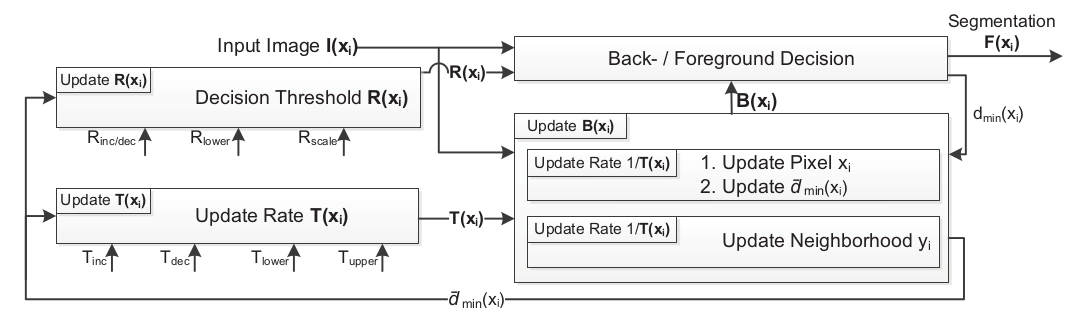
\includegraphics[width=\textwidth]{Figures/PBAS_state_machine.png}
    \caption{PBAS state machine.}
\end{figure*}

The background model $B(x_i)$ is defined by an array of N recently observed pixel values:
\begin{equation}
\mathbf{B}(x_i) = \{B_1(x_i),...,B_k(x_i),...,B_N(x_i)\}
\end{equation}
A pixel $x_i$ is decided to belong to the background, if its
pixel value $I(x_i) $ is closer than a certain decision threshold
$R(x_i)$ to at least $K$ of the $N$ background values. Thus,
the foreground segmentation mask is calculated as:
\begin{equation} \label{eq:F}
F(x_i) = \begin{cases} 1,& \#\{dist(I(x_i), B_k(x_i)) < R(x_i)\} < K \\0 &else\end{cases}
\end{equation}
$F = 1$ implies foreground. The decision involves two parameters: the distance threshold $R(x_i)$, which is defined for each pixel separately and which can change dynamically, and the minimum number $K$, which is a fixed global parameter. The function $dist$ is a distance measure, as explained in equation (\ref{eq:dist}).
\paragraph{Update B}
The background model is only updated for those pixels that
are currently background (i.e. $F(x_i) = 0$).
Updating means that for a certain index $k \in \{1...N \}$ (chosen uniformly at random), the corresponding background model value $B_k(x_i)$ is replaced by the current pixel value $I(x_i)$.
This allows the current pixel value to be ”learned” into the background model. This update, however, is only performed with probability $p = 1/T(x_i)$. Otherwise no update
is carried out at all. Therefore, the parameter $T(x_i)$ defines the update rate. The higher $T(x_i)$ the less likely a pixel will be updated.
It is also updated (with probability $p = 1/T(x_i)$) a randomly chosen neighboring pixel $y_i \in N(x_i)$. Thus, the background model $B_k(y_i)$ at this neighboring pixel is replaced by its current pixel value $V(y_i)$.
\paragraph{Update R}
To change the decision treshold $R(x_i)$ is saved an array of recently observed pixel values in the background model $B(x_i)$, we also create an array $\mathbf{D}(x_i) = \{D_1(x_i ),...,D_N(x_i)\}$ of minimal decision distances. Whenever an update of $B_k(x_i)$ is carried out, the currently observed minimal distance:
\[ d_{min}(x_i) = min_k \{dist(I(x_i), B_k(x_i))\} \] is written to this array: $D_k(x_i) \leftarrow d_{min}(x_i)$. Thus, a history of minimal decision distances is created. The average of these values $\overline{d}_{min}(x_i) = \frac{1}{N} \sum_k D_k(x_i)$ is a measure of the background dynamics. Thanks to that, the decision threshold can be dynamically adapted as follows:
\begin{equation} \label{eq:R}
R(x_i)=\begin{cases} R(x_i)\cdot(1-R{inc/dec}) &if\ R(x_i)> \overline{d}_{min}(x_i)\cdot R_{scale} \\ R(x_i)\cdot (1+R{inc/dec}) &else  \end{cases}
\end{equation}
Here, $R_{inc/dec}$ and $R_{scale}$ are fixed parameters. This can be seen as a dynamic controller for the state variable $R(x_i)$.
\paragraph{Update T}
Independent of the foreground state $F(x_i)$, every object will be merged into the background depending on the learning parameter
$T(x_i)$. To alleviate the problem, the idea is to introduce a
(second) dynamic controller for $T(x_i)$ following the assumption that pixels are mostly wrongly classified as foreground in areas of high dynamic background the strength of the adjustment in the controller can be adapted using the dynamic estimator $\overline{d}_{min}(x_i)$. So can be defined:
\begin{equation}
T(x_i)=\begin{cases} T(x_i)+\frac{T_{inc}}{\overline{d}_{min}(x_i)} &if \ F(x_i)=1 \\ T(x_i)-\frac{T_{inc}}{\overline{d}_{min}(x_i)} &if \ F(x_i)=0 \end{cases}
\end{equation}
$T_{inc}$ and $T_{dec}$ are fixed parameters. Are also defined $T_{lower}$ and $T_{upper}$ such that the values can not go out of a specific bound.
\paragraph{Distance computation}
The quantity $ dist(I(x_i),B_k(x_i)) $ is computed as:
\begin{equation} \label{eq:dist}
\frac{\alpha}{\overline{I^m}}|I^m(x_i) - B_k^m(x_i)| + |I^v(x_i) - B_k^v(x_i)|
\end{equation}
where $m$ indicates the gradient magnitude and $v$ the pixel intensity value. $\overline{I_m}$ is the average gradient magnitude over the last observed frame. Thus, the fraction $\frac{\alpha}{\overline{I^m}}$ weighs the importance of pixel values against the gradient magnitude.

\section*{Experiments}

In this section, we first report the results obtained by varying the main model parameters. We also include the adopted settings that perform best in our scenario. Then, we show some real-case usages of the algorithm, comparing different environmental conditions that we found in 24/24h live videos.

\subsection{Hyperparameters}

\subsection*{N}
$N$ represents how many matrices are kept in memory to model the background.
Each of them stores the history of pixels values (so $N$ entries).
The greater, the more complex backgrounds can be handled, but at the cost of heavier
computation.
\begin{figure}[!t]
\centering
\subfloat[][N = 2]{
    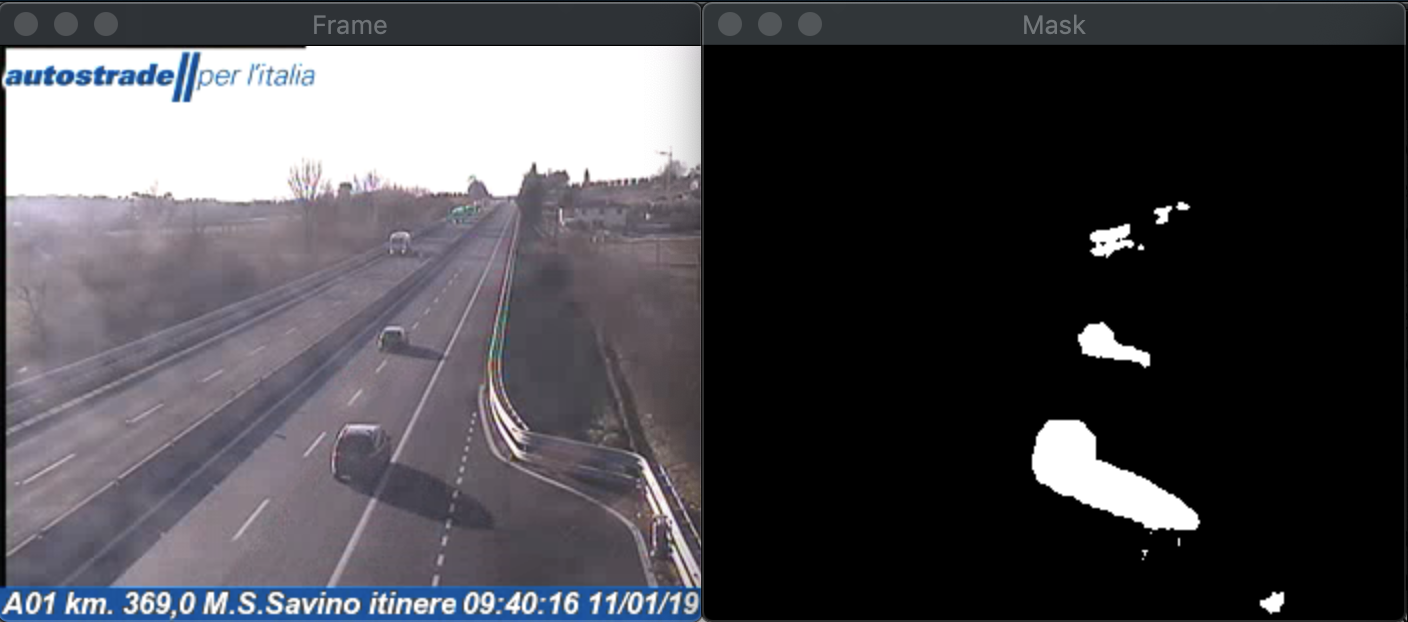
\includegraphics[width=0.45\textwidth]{Figures/N2.jpg}
    %\label{fig:N2}
}
\newline
\subfloat[][N = 10]{
    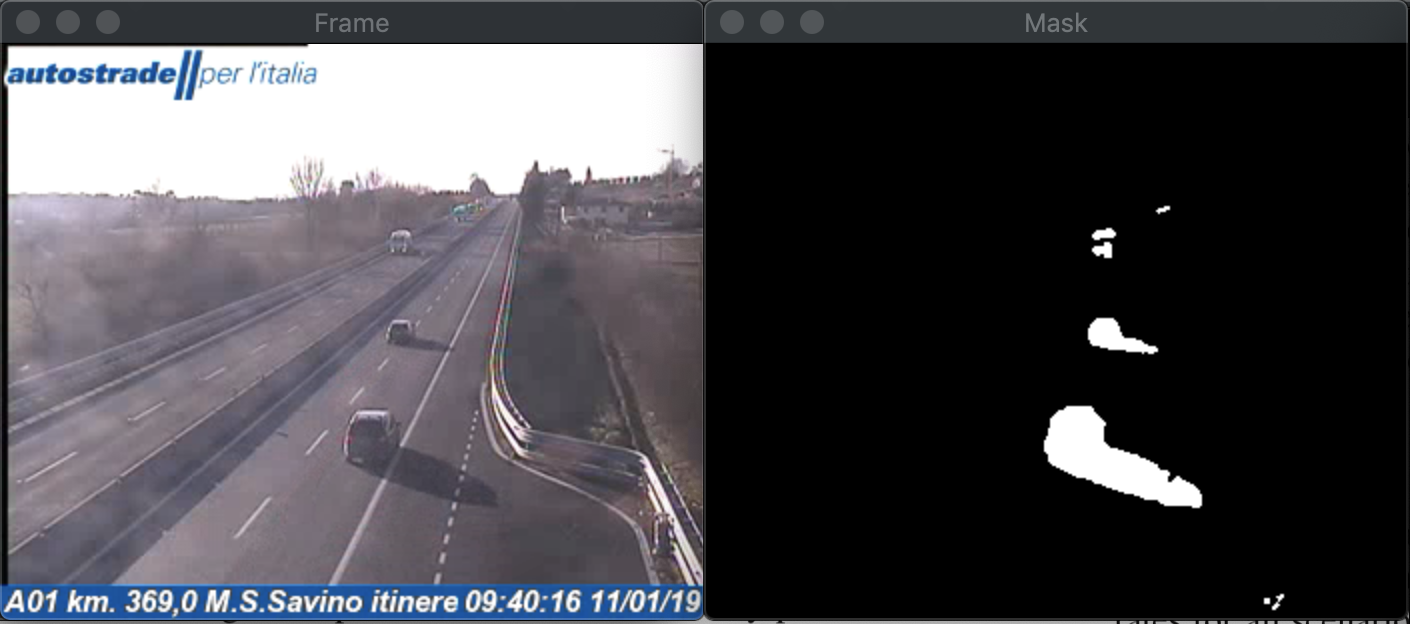
\includegraphics[width=0.45\textwidth]{Figures/N10.jpg}
}
\newline
\subfloat[][N = 20]{
    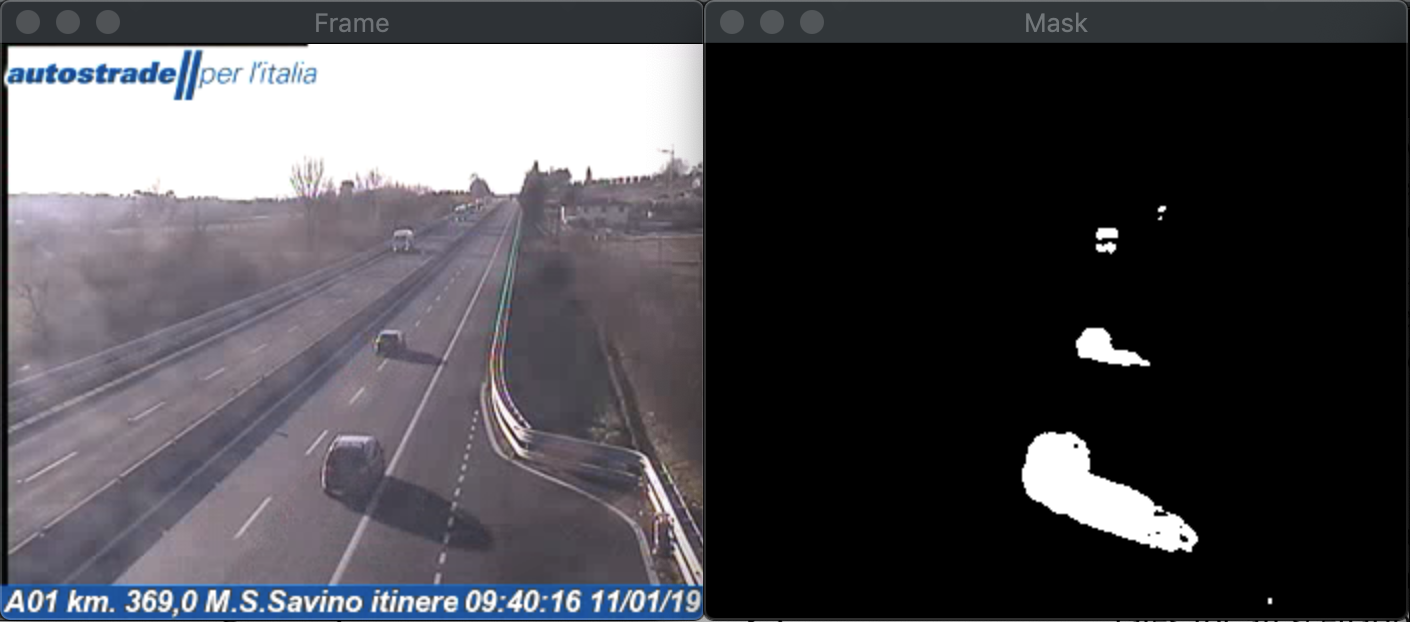
\includegraphics[width=0.45\textwidth]{Figures/N20.jpg}
}
\caption{We can see the poor mask of the cars on the left road when $N=2$, and the
accurate mask of the lines on the front right when $N=20$.}
\end{figure}


\subsection*{K}
$K$ tells the number of samples from $B$ that have to be closer than $R$ in order to
classify the pixel as background. The higher, the more difficult for a pixel to be
classified as background.
\begin{figure}[!t]
\centering
\subfloat[][K = 1]{
    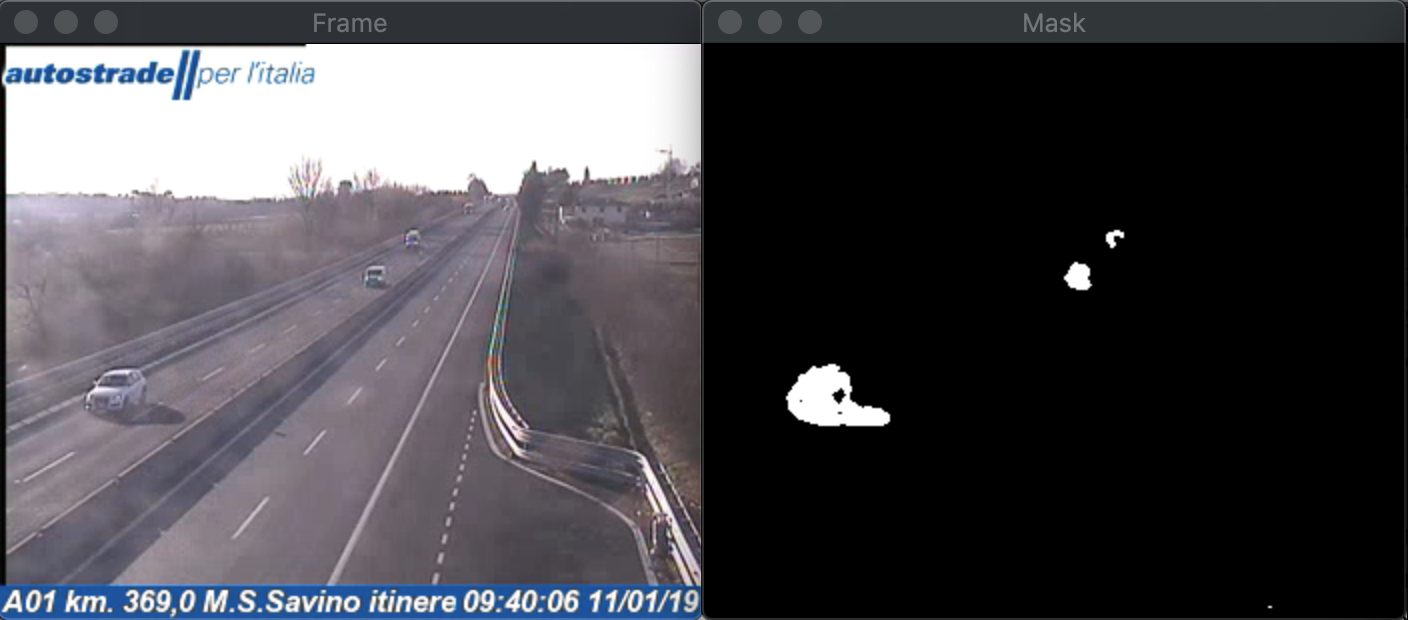
\includegraphics[width=0.45\textwidth]{Figures/K1.jpg}
}
\newline
\subfloat[][K = 2]{
    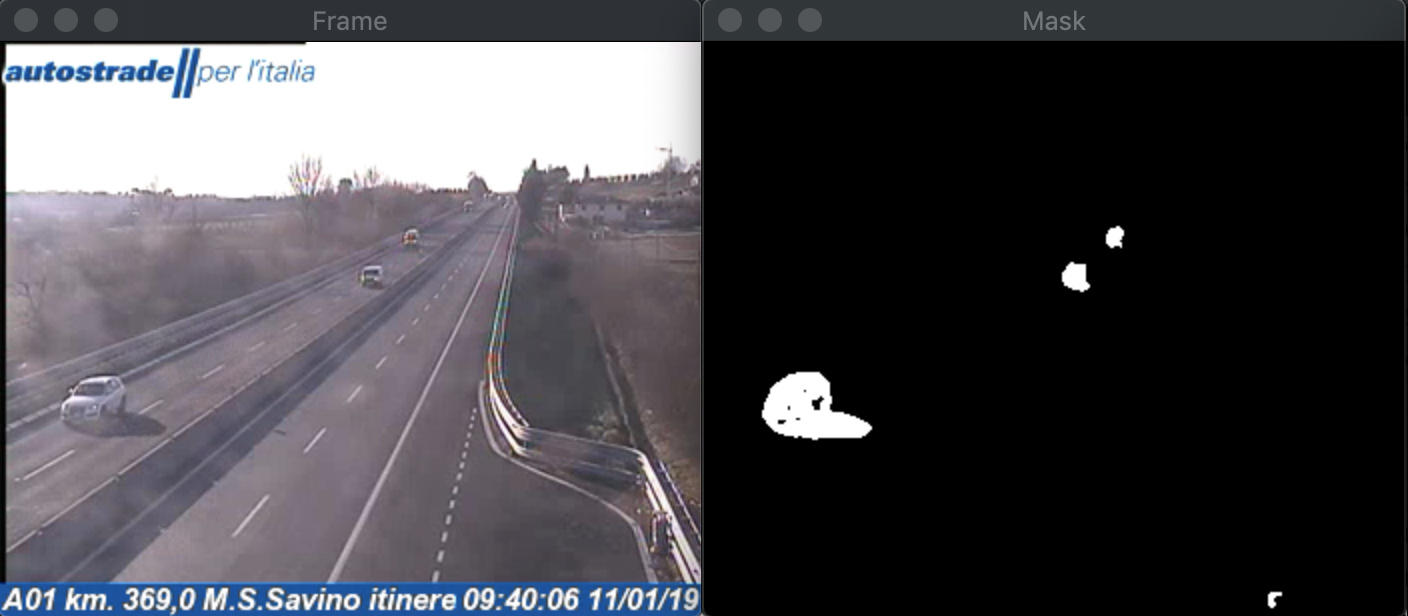
\includegraphics[width=0.45\textwidth]{Figures/K2.jpg}
}
\newline
\subfloat[][K = 4]{
    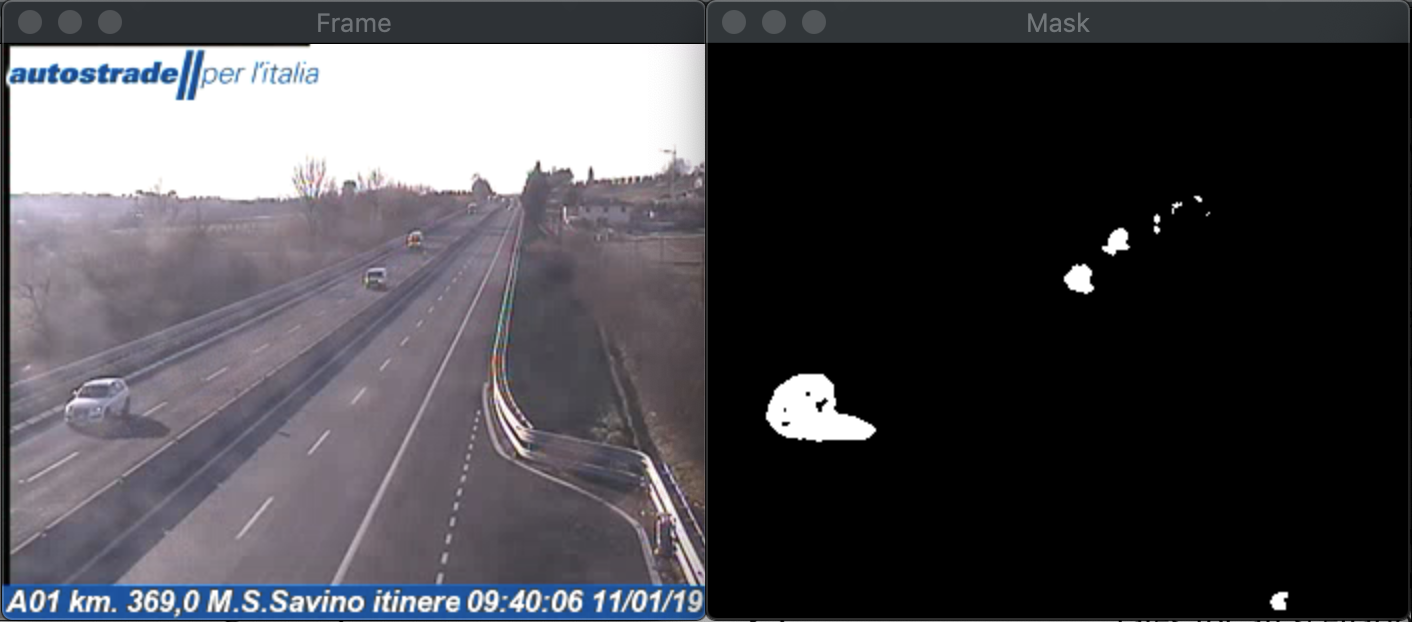
\includegraphics[width=0.45\textwidth]{Figures/K4.jpg}
}
\caption{Setting $K$ too high brings to classify many pixels as foreground, with the risk of false positives.}
\end{figure}

\subsection*{T}
The controller $T(x_i)$ associated to each pixel, is introduced with the idea to change dinamically the learning rate associated to each pixel based on its classification. It is slowly increased when the pixel is classified as background and slowly decreased when the pixel is classified as foreground. That leads to have a better foreground detection for multiple reasons: in case of highly dynamic background (i.e. big $\overline{d}_{min}(x_i)$), the learning parameter $T(x_i)$ stays constant or only slightly changes. In this case of highly dynamic background, erroneously detected foreground will not remain for long, because the probability to update $p = 1/T(x_i)$ does not reach
zero too fast. \newline
In the other ideal case of a fully static background, a classification as foreground is quite solid so $T(x_i)$ can be rapidly increased or decreased. \newline
$T_{upper}$, $T_{lower}$: control respectively the lowest and the highest probability of updating a pixel and putting it in the background model $B$. \newline
$T_{inc}$, $T_{dec}$: are fixed parameters and control the update of the controller T of each pixel.\newline
Since one of the objective of the work is to have a robust classification of the foreground objects, we want to find the best values for the T parameters such that an object if classified as foreground stay as it for the longest period of time. 
\begin{figure}[!t]
    \centering
    \subfloat[][$T_{inc}$ = 1]{
        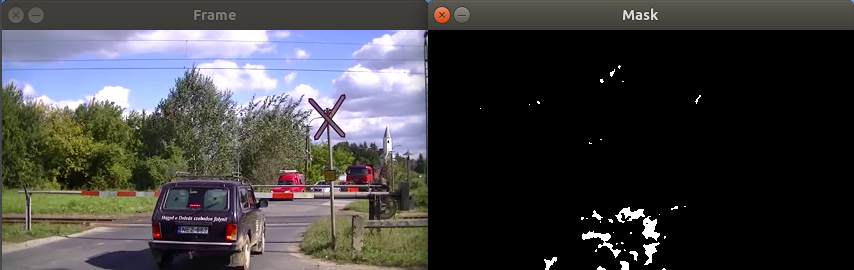
\includegraphics[width=0.45\textwidth]{Figures/T_inc_1.png}
    }
    \newline
    \subfloat[][$T_{inc}$ = 5]{
        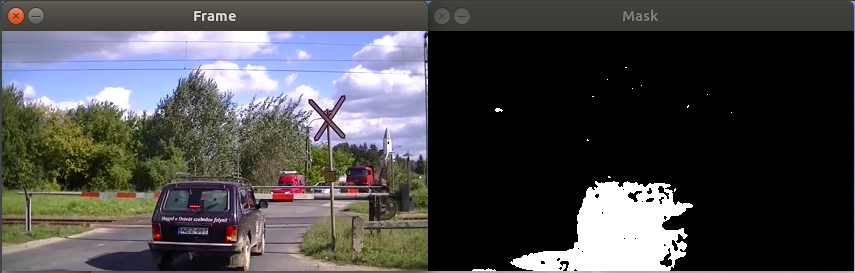
\includegraphics[width=0.45\textwidth]{Figures/T_inc_5.png}
    }
    \caption{Have an higher $T_{inc}$ means decreasing faster the probability that a pixel is included in the background model once it is classified as foreground. Clearly visible in the two image reporting a car stopped for $30s$.}
\end{figure}


\subsection*{R}
Eq (\ref{eq:R}) is similar to the equation of a pure proportional controller.
In this case the $R(x,y)$ has to follow $d_{minavg}(x,y)R_{scale}$. So:
\begin{itemize}
    \item $R_{incdec}$: it can be seen as the propositional constant of the controller: setting too high can lead to oscillation around the target and even to divergence. Setting too low leads to slow convergence to the target values, making the algorithm too slow to adapt to dynamic backgrounds.
    \item $R_{scale}$: tells how much the algorithm is sensitive, in fact it is a direct
    control of the threshold. Setting too high it leads to really few false positives
    but also decreases true positives; setting too low, will increase false positives.
    \item $R_{lower}$: sets a limit on how much $R$ can decrease its value. Setting it too
    low will lead to a lot of false positives,
   especially in zones that are changing their values of high amounts due to noise. Setting too
    high it will reduce true positives. So its value should be led by the
    video quality, more than the application domain.
\end{itemize}
\begin{figure}[!t]
    \centering
    \subfloat[][$R_{scale}$ = 5]{
        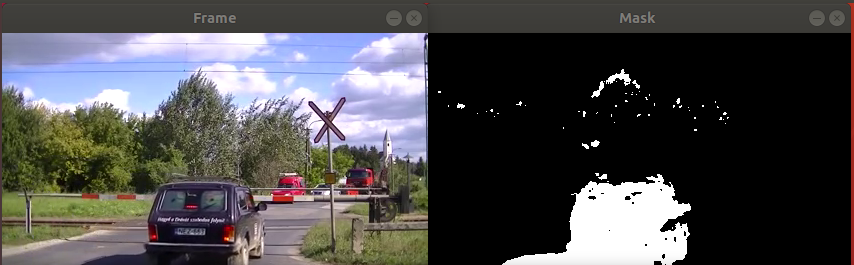
\includegraphics[width=0.45\textwidth]{Figures/R_scale5.jpg}
    }
    \newline
    \subfloat[][$R_{scale}$ = 15]{
        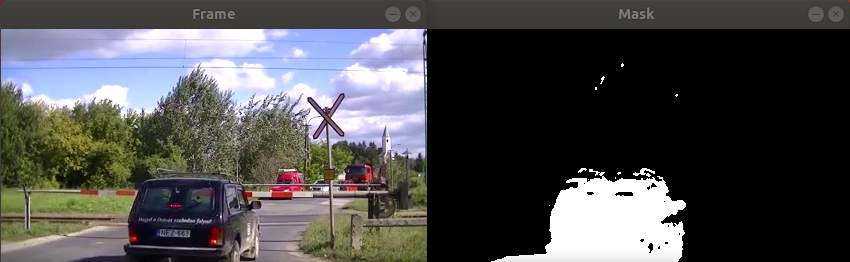
\includegraphics[width=0.45\textwidth]{Figures/R_scale15.jpg}
    }
    \newline
    \subfloat[][$R_{scale}$ = 50]{
        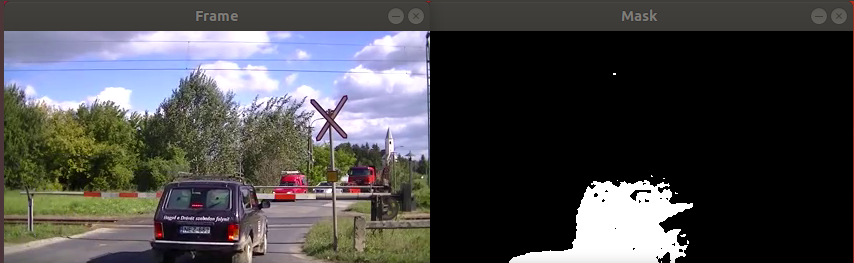
\includegraphics[width=0.45\textwidth]{Figures/R_scale50.jpg}
    }
    \caption{As $R_{scale}$ grows the tree leaves that are waved by the wind are not detected
anymore as foreground but also a part of the car is lost.}
\end{figure}

\subsection*{$\bm{\alpha}$}
From eq (\ref{eq:dist}) we see that $\alpha$ tells how much to weight the image gradients
with respect to the image values in the distance computation.
%\begin{figure}[!t]
%    \centering
%    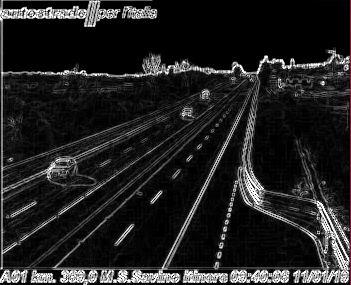
\includegraphics[width=0.45\textwidth]{Figures/gradients.jpg}
%    \caption{Gradients}
%    \label{fig:gradients}
%\end{figure}
The image gradients give a good cue to distinguish the street from the cars
(image absolute values are not, since many cars have almost the same color of the
street). So alpha should be set high, in order to take into consideration this fact.
But notice that setting too high will lead to noisy masks, especially with noisy
videos that have small variations of the gradient from frame to frame.
\begin{figure}[!t]
    \centering
    \subfloat[][$\alpha$ = 0]{
        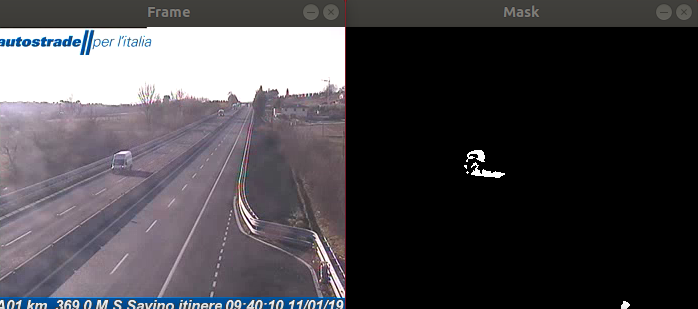
\includegraphics[width=0.45\textwidth]{Figures/alpha0.jpg}
    }
    \newline
    \subfloat[][$\alpha$ = 10]{
        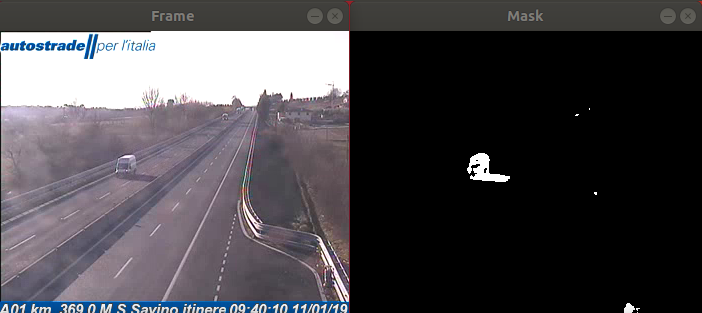
\includegraphics[width=0.45\textwidth]{Figures/alpha10.jpg}
    }
    \newline
    \subfloat[][$\alpha$ = 20]{
        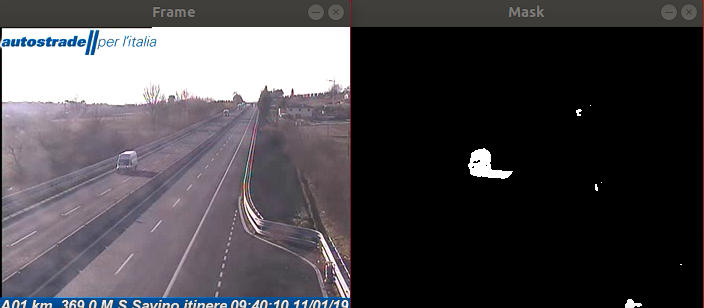
\includegraphics[width=0.45\textwidth]{Figures/alpha20.jpg}
    }
    \newline
    \subfloat[][$\alpha$ = 50]{
        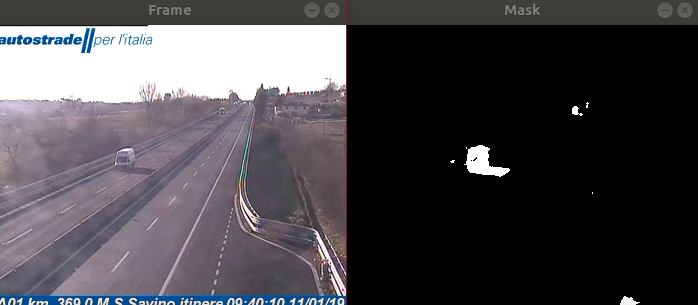
\includegraphics[width=0.45\textwidth]{Figures/alpha50.jpg}
    }
    \caption{The influence of the image gradients. In \textbf{(a)} is reported the mask not considering the gradients ($\alpha = 0$). Going toward the bottom, we see the good influence on the detection, but we also witness an increase of the noise.}
\end{figure}

\subsection{Post-processing}
To refine the performance of the algorithm, a median-filter is applied to the final mask using a square kernel. Since the values of the pixels can be 0 or 255 this is equivalent to perform a majority voting among the kernel's pixels to decide the value of the middle one. That has shown to reduce the noise on the final mask and in the meanwhile generate more connected components (Figure \ref{fig:median}). The size chosen for the kernel after different experiments is $5\times 5$.

\begin{figure} 
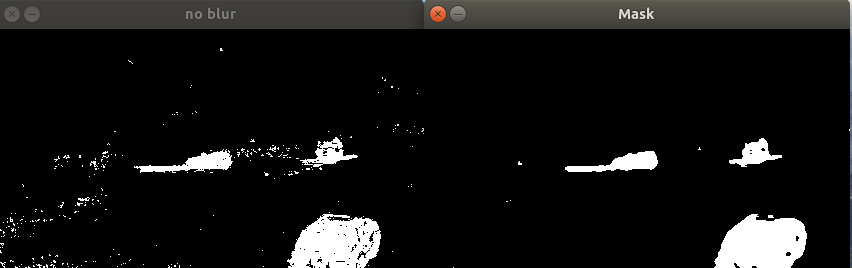
\includegraphics[width=\linewidth]{Figures/median_blur.png}
\caption{Comparison between output whitout post-processing and with median-blur post-processing}
\label{fig:median}
\end{figure}


\subsection{Optimal Setting}
The proposed method has a multitude of tunable parameters, their values have been chosen focusing the attention on having an algorithm robust to changing on weather condition and capable of identifying foreground object even if they stay steady for a period of time (e.g. cars stopped to a traffic light), still guaranteeing a real time behaviour. \newline
Experimental results have shown that the optimal parameters are the following:
\begin{itemize}
\item $N = 30:$ The number of components of the
background model. Increasing the value of this parameter let the algorithm be more robust to noise, but at the same time, increase a lot the time complexity. The value has been choosen considering the previous tradeoff.
\item $K = 3:$ The number of components that have to be closer than $R(x_i)$ in order to set the pixel to be background. We raise it to 3 (instead of 2) because we want to be stricter in the background classification, since cars are often segmented only near the borders and masks present holes in the central area, probably because the car color is matched with some previous background pixels.
\item $R_{incdec} = 0.05:$ Proportial constant of the controller for the variable $R(x_i)$. The value 0.05 leads to pretty fast adaptation to the target value of $R(x_i)$ (in more or less 30 frames the target is reached). Considering that our target are long periods of time there is no reason to raise it.
\item $R_{lower}=18:$ Lower bound of the decision threshold. It has been left to the value proposed in the original paper, since we found that raising it would lead to a significant decrease in true positive and lowering it would let too much noise in.
\item $R_{scale}=2:$ Scaling factor in the controller for the decision threshold. Setting it to 2 has shown to let the algorithm recognize better the foreground object while introducing very low noise.
\item $T_{dec} = 0.05:$ If $x_i$ is background, $T_{dec}$ is the rate at which $T(x_i)$ is decreased.
\item $T_{inc} = 5:$ If $x_i$ is foreground, $T_{inc}$ is the rate at which $T(x_i)$ is increased. These parameter has shown to be very important to keep classified as foreground pixels associated to objects that have stopped their movement. Increasing it to 5 from the proposed value of 2 reduces faster the probability to put a steady foreground object in to one of the N components of the background model.
\item $T_{lower}= 2:$ Lower bound of $T(x_i)$.
\item $T_{upper}= 200:$ Upper bound of $T(x_i)$.
\item $\alpha = 20:$ Weight to give to image gradients. The proposed value is high because this shows to be a good cue for distinguishing car objects.
\end{itemize} 

\subsection{Long Period Experiments}
Since our goal is traffic monitoring 24/7, it is important to ensure that the algorithm can adapt as time passes to different light conditions, environmental changes, and traffic intensity variations. In order to do this, we let the algorithm run on ninety minutes long videos recording smooth light transitions (from day to night and viceversa), rough changes of environmental conditions and variations of traffic intensity. Experiments show that the algorithm adapts without any problem in those scenarios. This makes us believe that also in a real 24/7 scenario there wouldn't be any adaptation problems. However, this behaviour is better than expected: looking at how the PBAS works, we can notice that the state (that is the values of the variables) would change in the same way during the starting iterations as it would after one day of non-stop run.

\begin{figure}[!t]
    \centering
    \subfloat[][00:00:30]{
        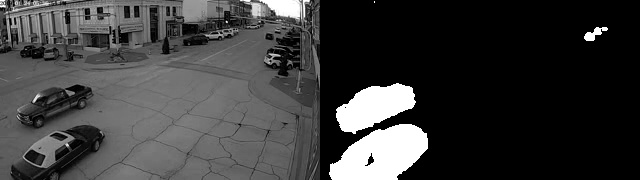
\includegraphics[width=0.45\textwidth]{Figures/sunset_1.jpg}
    }
    \newline
    \subfloat[][00:30:00]{
        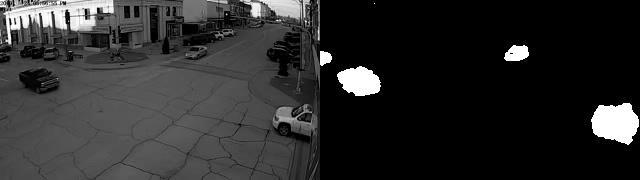
\includegraphics[width=0.45\textwidth]{Figures/sunset_2.jpg}
    }
    \newline
    \subfloat[][00:45:00]{
        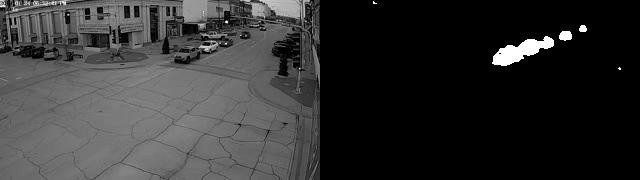
\includegraphics[width=0.45\textwidth]{Figures/sunset_3.jpg}
    }
    \newline
    \subfloat[][01:10:00]{
        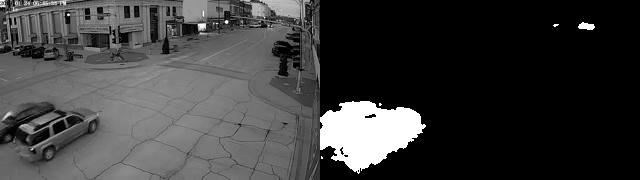
\includegraphics[width=0.45\textwidth]{Figures/sunset_4.jpg}
    }
    \newline
    \subfloat[][01:29:30]{
        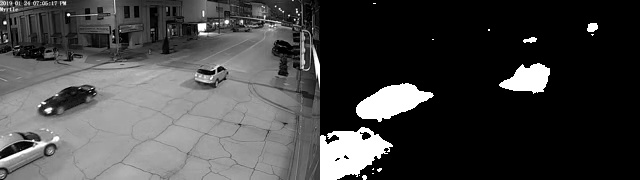
\includegraphics[width=0.45\textwidth]{Figures/sunset_5.jpg}
    }
    \caption{It is shown how the algorithm adapts to change of lighting conditions, in particular when the sun sets.}
\end{figure}


\begin{figure}[!t]
    \centering
    \subfloat[][00:01:00]{
        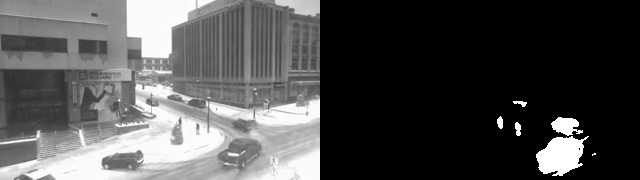
\includegraphics[width=0.45\textwidth]{Figures/snow_60.jpg}
    }
    \newline
    \subfloat[][00:26:00]{
        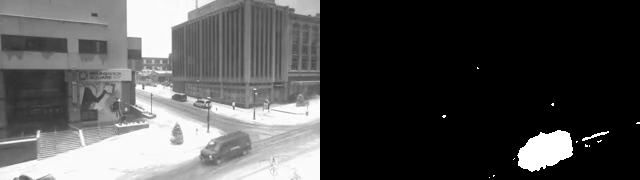
\includegraphics[width=0.45\textwidth]{Figures/snow_1561.jpg}
    }
    \newline
    \subfloat[][00:35:00]{
        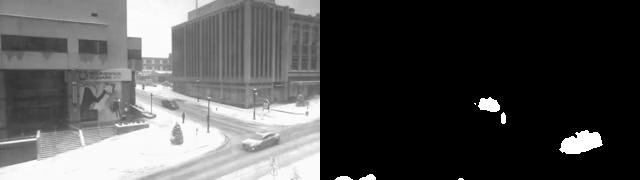
\includegraphics[width=0.45\textwidth]{Figures/snow_1921.jpg}
    }
    \newline
    \subfloat[][01:04:00]{
        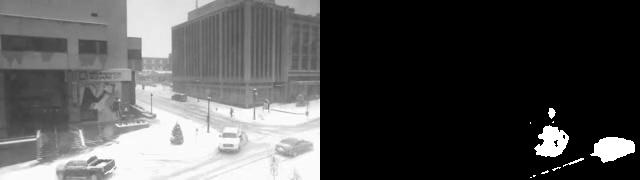
\includegraphics[width=0.45\textwidth]{Figures/snow_3850.jpg}
    }
    \newline
    \subfloat[][01:29:00]{
        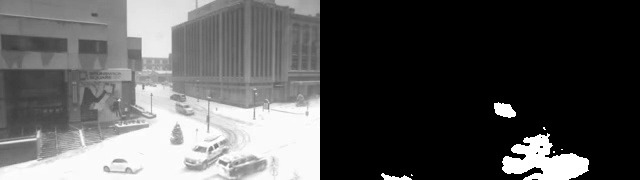
\includegraphics[width=0.45\textwidth]{Figures/snow_5377.jpg}
    }
    \caption{It is shown how the algorithm adapts to change of enviromental conditions. In this case it starts snowing, therefore the road gets dirtier than it was when the video started.}
\end{figure}

\begin{figure}[!t]
    \centering
    \subfloat[][00:06:00]{
        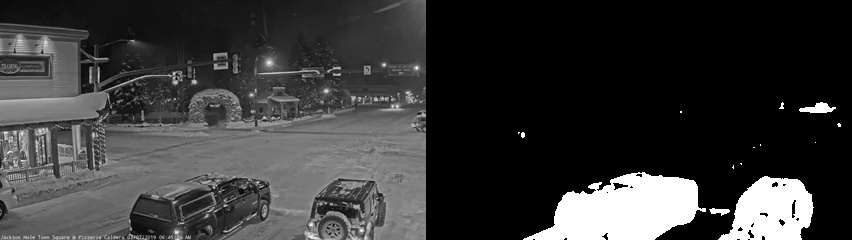
\includegraphics[width=0.45\textwidth]{Figures/24h_1.jpg}
    }
    \newline
    \subfloat[][00:28:00]{
        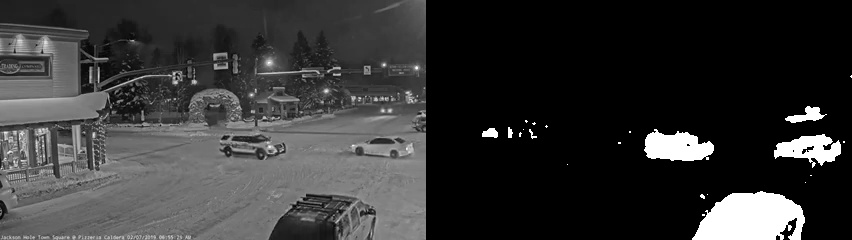
\includegraphics[width=0.45\textwidth]{Figures/24h_2.jpg}
    }
    \newline
    \subfloat[][00:45:00]{
        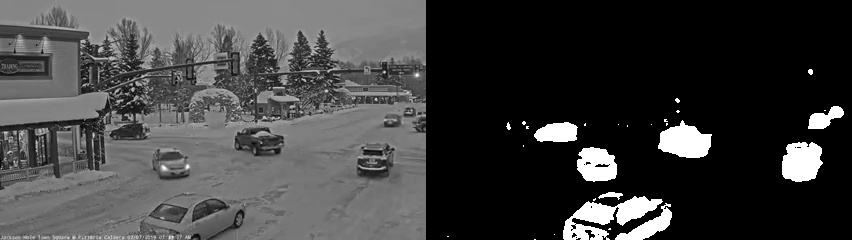
\includegraphics[width=0.45\textwidth]{Figures/24h_3.jpg}
    }
    \newline
    \subfloat[][01:00:00]{
        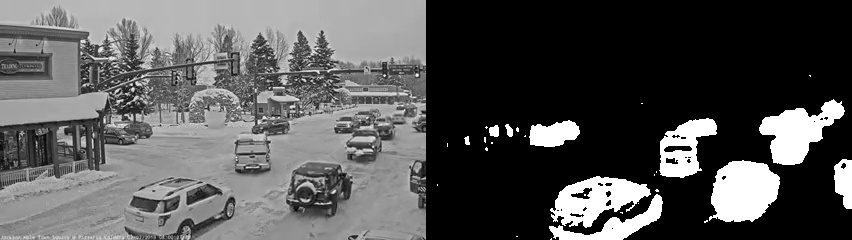
\includegraphics[width=0.45\textwidth]{Figures/24h_4.jpg}
    }
    \newline
    \subfloat[][01:23:00]{
        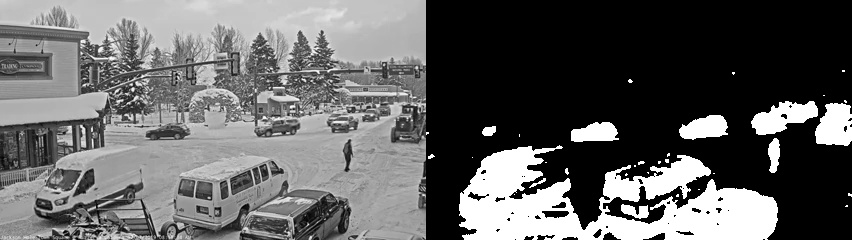
\includegraphics[width=0.45\textwidth]{Figures/24h_5.jpg}
    }
    \caption{It is shown how the algorithm adapts to change of lightining and traffic conditions during a 1h and 30 min video sample.}
\end{figure}

\section*{Improvements}

\subsection*{RGB vs Grey}
We have experimented with a version of the algorithm working just on grey scale images and with one exploiting also color informations. The grey one is implementing exactly all the steps described in \ref{subsect:PBAS}. The RGB version runs the greyscale version for each of the three channels in parallel threads and then the final mask is computed as the logical-OR of the three masks obtained from the three channels.
Experiments show that the RGB version has slightly better cars detection capabilities, but obviuosly computationally heavier. We could not be able to try with a 4-core CPU, but in theory this can bring times down to the grayscale version, since the 3 channels can be computed quickly expoliting parallelism.

\begin{figure}[!t]
    \centering
    \subfloat[][Grey]{
        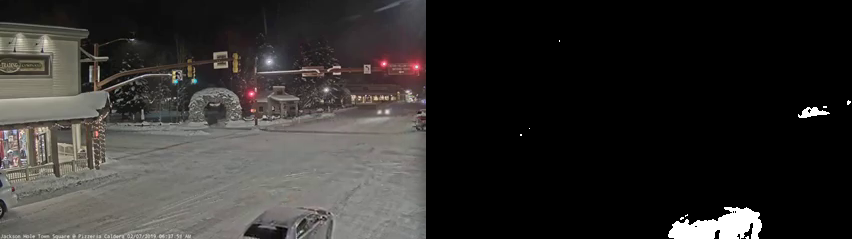
\includegraphics[width=0.45\textwidth]{Figures/grey.png}
    }
    \newline
    \subfloat[][RGB]{
        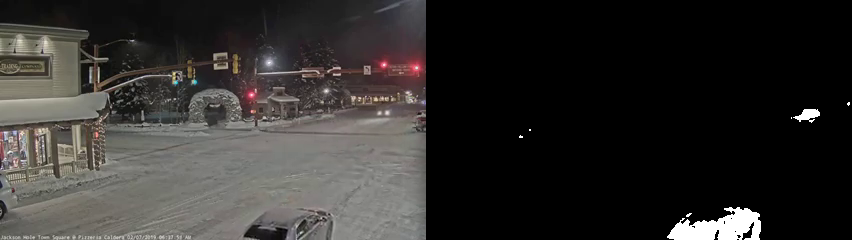
\includegraphics[width=0.45\textwidth]{Figures/rgb.png}
    }
    \newline
    \subfloat[][Gray and RBG on intermittent motion video]{
        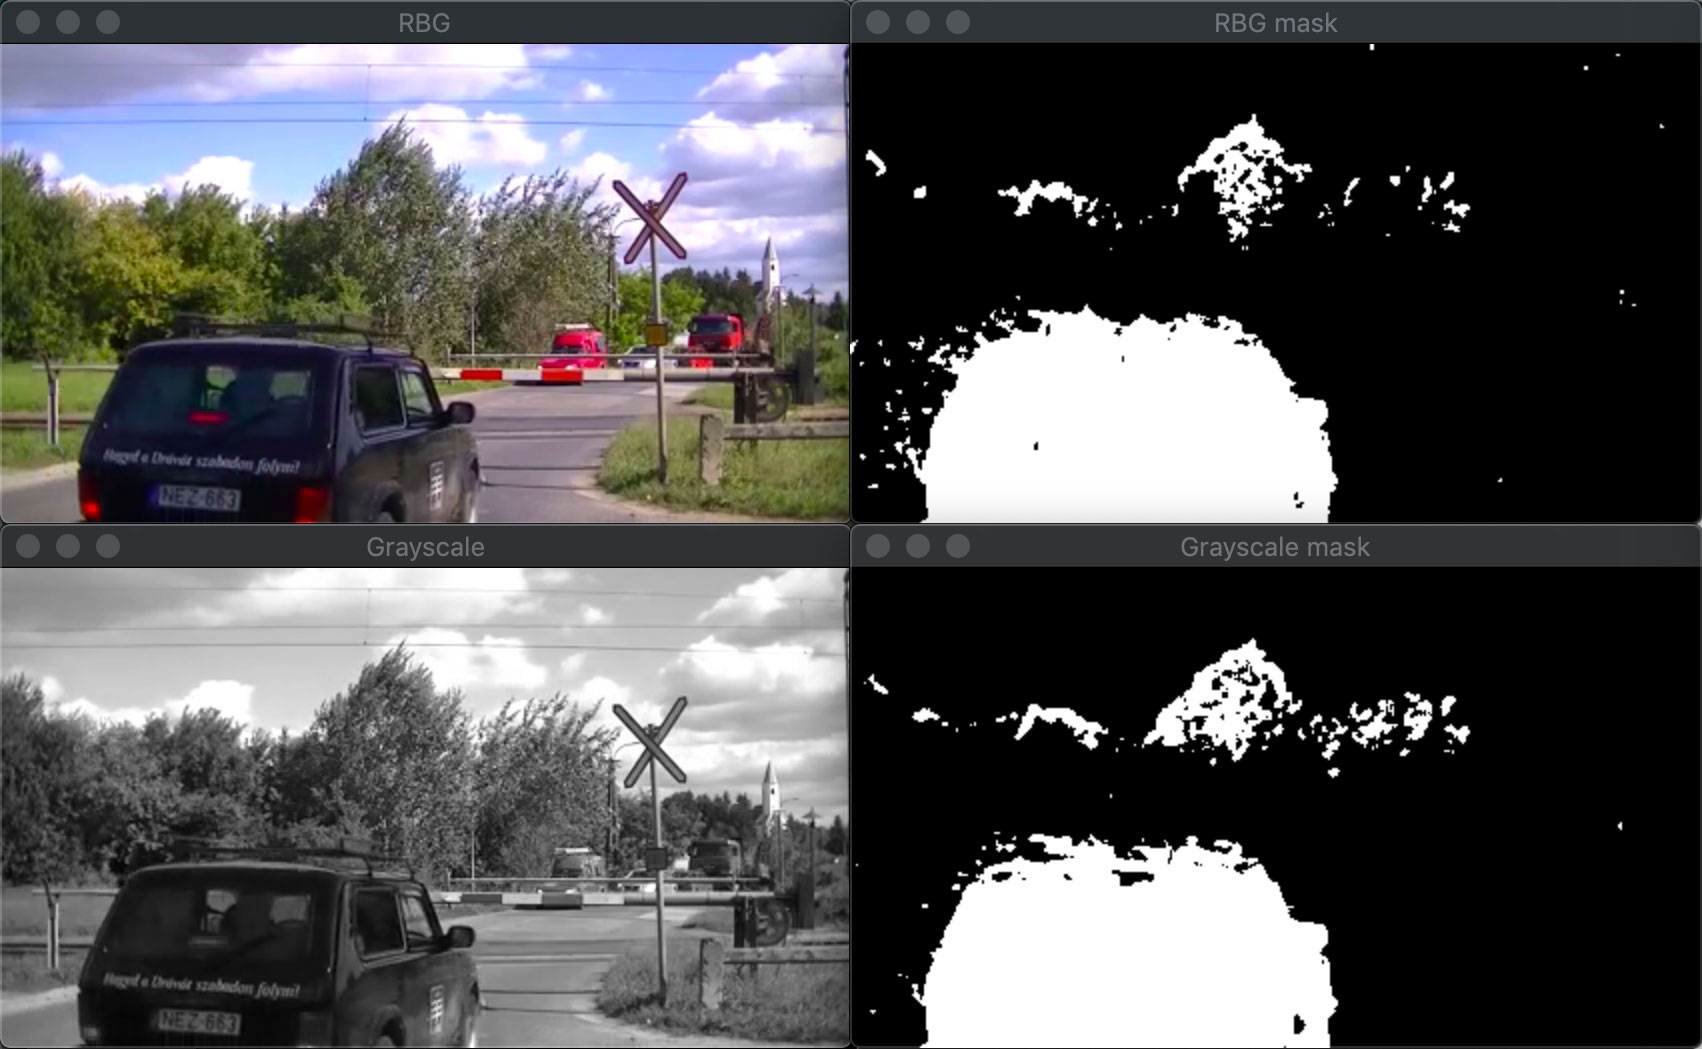
\includegraphics[width=0.45\textwidth]{Figures/rgbvsgray.jpg}
    }
    \caption{Comparison between grayscale and RBG versions of the PBAS. As we see, there are some differences in the detection accuracy. In good light situations, e.g. sunny days, the RGB version provide better foreground masks and less noise.}
\end{figure}

\subsection*{Optical flow analysis}
The algorithm is fully based on the variations of a pixel intensity over time. This cannot be enough in some situations to provide a correct segmentation, for example, we noticed that a traffic light is classified as a foreground element because it emits 3 different light colors that vary a lot from each other and very quickly from frame to frame (this problem has a more evident impact especially when using 3-channels videos). We can resort to optical flow to detect this kind of issues: in fact, optical flow provides a measure of the motion of pixels in consecutive frames, so in the previous case the flow of pixels in the area of the traffic light will not be present. So, we can discriminate pixels that have flow and pixels that have not, changing different parameters of the PBAS for these two categories.

We built a model to determine which pixels had an "active" flow in the past, and in some sense these pixels represents road areas subject to traffic. We adopted the Farneback dense optical flow algorithm to get the flow of each pixel of the frame. Then, we checked which pixels had a flow magnitude over a certain threshold $W_{min}$ and we stored this information in a history of $L$ previous samples. If the magnitude of the flow was greater then $W_{min}$ for L consecutive frames, than the pixel is classified as "flow-active". For all the "flow-active" pixels, we applied some ad-hoc adjustments for the PBAS parameters, in particular we decremented the update frequency $T$ by a constant to penalyze the chances of those pixels to be inserted in the background model. Further changes can be done, however are out of the scope of this project.

\begin{figure}[!t]
    \centering
    \subfloat[][No optical flow]{
        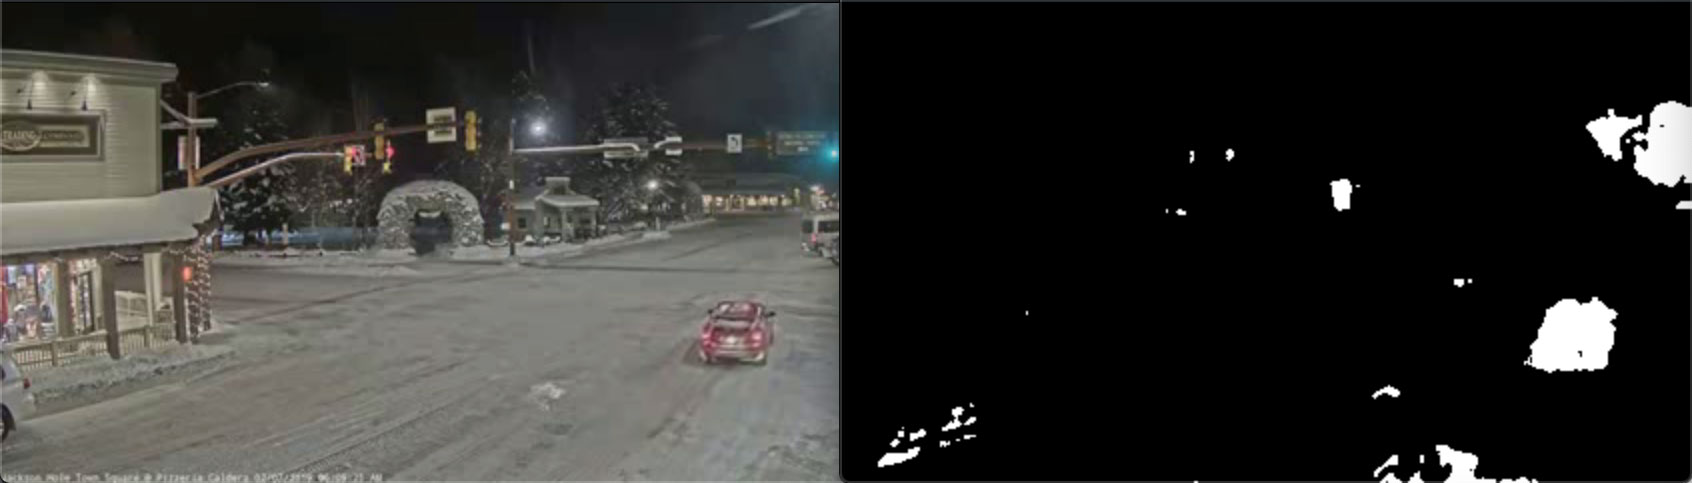
\includegraphics[width=0.45\textwidth]{Figures/noflow.jpg}
    }
    \newline
    \subfloat[][Optical flow]{
        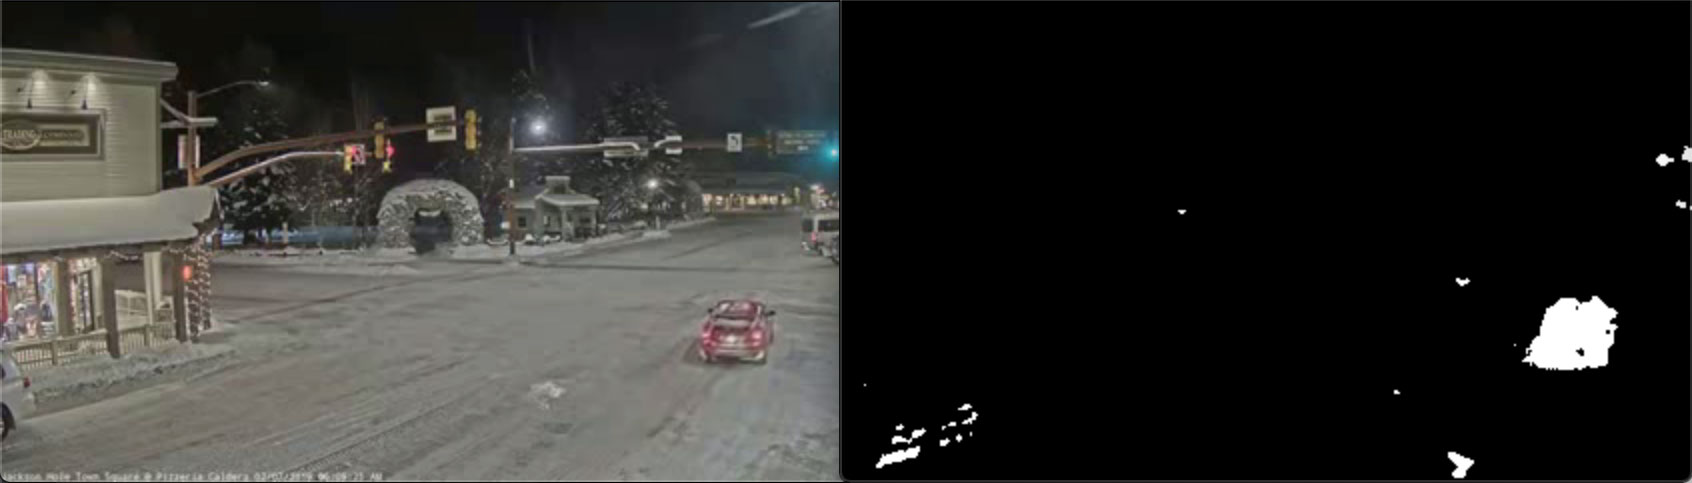
\includegraphics[width=0.45\textwidth]{Figures/flow.jpg}
    }
	\caption{Optical flow version compared with the naive version. The former one is aware of areas that have an "active flow" and put those pixels in the background model less frequent, e.g. the traffic light on the right.}
\end{figure}

\subsection*{Improvements and computational impact}
We report here the time (in ms) required to analyze one frame using our implementation of the PBAS algorithm, with and without the proposed improvements. The algorithm has been run on a Macbook Pro mounting an Intel Core i5 2.3 GHz and 8 GB 2133MHz of LPDDR3 RAM, using as input 426x240 frames. Performances can drastically be raised by running it on a 4-core CPU (that is able to handle the 3 threads of the RBG channels in parallel) or on a GPU.

\begin{table}[]
\begin{tabular}{l|c}
    Algorithm                                     & Average time \\
    \hline
    PBAS on grayscale video                       & 90ms         \\
    PBAS on RBG video                             & 180ms        \\
    PBAS on RBG video with optical flow   & 200ms        
\end{tabular}
\end{table}

\section*{Conclusion}
We have provided a background subtraction system based on the PBAS algorithm. The system is meant to work real time in traffic surveillance scenarios, also under challening environmental conditions and heavy traffic, 24/7. In order to do this, the general purpose PBAS algorithm was studied and the hyperparameters were adapted in order to perform best in this particular scenario. We have validated our work by visual inspection in particular and challenging situations, with long videos with environmental and traffic conditions changing over time. We further experimented with noise removal methods and we tried to exploit motion informations. Future work can be done in this direction, until arriving to a precise classification of noise and errors in the mask detected. Still, the system as it is now can be employed as a preprocessing step for many anomaly detection applications, such as car accidents, cars going in the wrong direction and people crossing the road.